\documentclass[11pt,a4paper]{article}
% rozmery stranky
\usepackage[left=1.5cm,text={18cm, 25cm},top=2.5cm]{geometry}
% cestina a fonty
\usepackage[czech]{babel}
\usepackage[utf8]{inputenc}
\usepackage[T1]{fontenc}
% dalsi balicky
\usepackage{graphicx}
\usepackage{enumitem}
\usepackage{indentfirst}
\usepackage{url}
\usepackage[bookmarksopen,colorlinks,plainpages=false,urlcolor=blue,
unicode,linkcolor=black]{hyperref}


\begin{document}

  \begin{titlepage}
    \begin{center}
      \Huge
      \textsc{Fakulta informačních technologií\\ Vysoké učení technické v~Brně}
      \vspace{100px}
      \begin{figure}[!h]
        \centering
        
\includegraphics[height=5cm]{logo}
      \end{figure}
      \\[50mm]
      \LARGE{Studie účelnosti zbudování vodní cesty Dunaj-Odra-Labe \,--\, 
             zadání č. 2}
      \vfill
    \end{center}
    \Large{Roman Blanco (xblanc01) \hfill 7.12.2014 \\
           Adam Jež (xjezad00)}
  \end{titlepage}

  \tableofcontents
  \newpage

  \section{Úvod}

    Cílem zadaného projektu bylo prostudovat zdroje, zabývající se účelností
    vybudování vodního koridoru Dunaj-Odra-Labe, a podle zjištěných údajů
    stanovit kvalifikovaný odhad roční poptávky po lodní přepravě mezi
    zvolenými uzly. 

    Součástí zadání bylo také navrhnout a implementovat model SHO
    (Systém hromadné obsluhy - IMS slide č. 139) dopravní cesty, včetně
    stavebních prvků.

    \subsection{Autoři}

      Autory projektu jsou Roman Blanco (xblanc01) a Adam Jež (xjezad00) \,--\,
      studenti 3. ročníku bakalářského studia na Fakultě Informačních
      technologii VUT v Brně. Prioritním zdrojem informací týkajících se
      zadaného tématu byly veřejně přístupné zdroje. Některé informace nám
      byly poskytnuty autory projektu zabývajícího se výstavbou koridoru.

    \subsection{Ověřování validity modelu}

      Ověřování validity modelu probíhalo pomocí experimentů, a to simulací ve
      virtuálním prostředí (Validace modelu - IMS slide č. 37). Ověřovalo se,
      zda modelová situace odpovídá reálné situaci, přičemž informace
      byly čerpány pouze z věrohodných zdrojů. Jelikož reálný systém,
      určený simulovaným modelem v současné době neexistuje, jako validní jsme
      model prohlásili na základě získaných informací

  \section{Rozbor tématu}

    Informace, potřebné pro úspěšnou implementaci byly vyhledány na veřejně
    přístupných stránkách na internetu. Problémem při využívání těchto zdrojů
    byla skutečnost, že mnoho informací, bylo uvedeno pouze v sumarizovaných
    hodnotách za období celého roku.  Pro některé hodnoty tak musel být použit
    kvalifikovaný odhad, podpořený údaji čerpanými ze statistik a dalších
    databází. Mimo již zmíněných veřejně přístupných webových stránek nám také
    často jako zdroj údajů posloužily diplomové či bakalářské práce. Níže je
    uveden souhrn hodnot, které jsme tímto způsobem získali:

    \noindent
    Hodnoty týkající se plavební komory:

    \begin{itemize}
      \item doba uzavření vrat plavební komory je 60 sekund
      \item doba otevření vrat plavební komory je 30 sekund
      \item doba vplutí do plavební komory je 516 sekund
      \item doba vyplutí z plavební komory je 355 sekund
      \item nízké plavební komora je taková, u níž výškový rozdíl mezi
            hladinami toku před a za komorou není větší než 12.5 m.
            Pokud plavební komora vyrovnává výšku hladiny přesahující 12.5 m,
            nazýváme ji vysokou plavební komorou
      \item napuštění nebo vypuštění 1 výškového metru "malé" plavební komory
            odpovídá doba 40 s
      \item napuštění nebo vypuštění 1 výškového metru  "velké" plavební komory
            odpovídá doba 25,45 s
    \end{itemize}

    \noindent
    Hodnoty,týkající se plavby v tunelu:

    \begin{itemize}
      \item bezpečná rychlost lodi při plavbě v tunelu je 2,22 m/s

      \item hranice, kdy se začne aplikovat seskupování je 3470 m [3]
            (Studie projektu - stana č. 48).
    \end{itemize}

    \noindent
    Hodnoty týkající se plavby v akvaduktu:

    \begin{itemize}
      \item rychlost při plavbě v tunelu je 2,77 m/s
      \item hranice, kdy se začne aplikovat seskupování je 2090 m
    \end{itemize}

    \noindent
    Obecné hodnoty při plavbě:

    \begin{itemize}
      \item rychlost plavby v kanálu je 3,33 m/s
      \item rychlost plavby po proudu toku řeky je 4,16 m/s
      \item rychlost plavby proti proudu toku řeky je 1,66 m/s
      \item maximální náklad lodi je 4000 tun
    \end{itemize}

    \noindent
    Dále jsme také pracovali s těmito informacemi:

    \begin{itemize}
      \item tunely jsou navrhovány jako jednolodní, tedy lodi v tunelu se
            nemohou pohybovat proti sobě. Lodě, které se chystají projet
            tunelem stejným směrem se mohou seskupit za účelem zrychlení plavby
            (Kniha - strana č. 157)
      \item je plánovana vodni trida Vb, kde mohou plout motorové nákladní lodě
            o nosnosti 2500 tun, nebo menší řičně-námořní lodě a tlačné
            soupravy s nosností 4000 tun
            (Kniha - strana č. 136)
      \item provoz plavebních komor je 24 hodin denně
            (Studie[3] - strana č. 38)
    \end{itemize}
        
    Jako prioritní zdroj informacím o plánované trase koridoru 
    nám velmi dobře posloužily volně
    dostupné materiály na internetové stránce projektu zabývajicího se
    problematikou koridoru Dunaj-Odra-Labe a také poskytnuta literatura[1] od
    těchtýž autorů.

    \subsection{Popis použitých postupů}

      V literatuře i na webových stránkách byly zobrazeny všechny části
      plánovaného koridoru s potřebnými údaji o trase:
      \begin{itemize}
        \item délky tunelů
        \item délky akvaduktů
        \item výškové rozdíly u plavebních komor
      \end{itemize}

      V knize byl také údaj určující, na kolikátém kilometru se stavební prvky
      nachází, z čehož bylo možné určit vzdálenosti mezi těmito prvky a tedy i
      délky úseků řek. (obrazek. č 1).  Označeny nebyly pouze polohy přistavů,
      tedy přibližná poloha přistavů byla odhadnuta pomocí blízkých stavebních
      prvků.

    \begin{figure}[ht!]
      \centering
      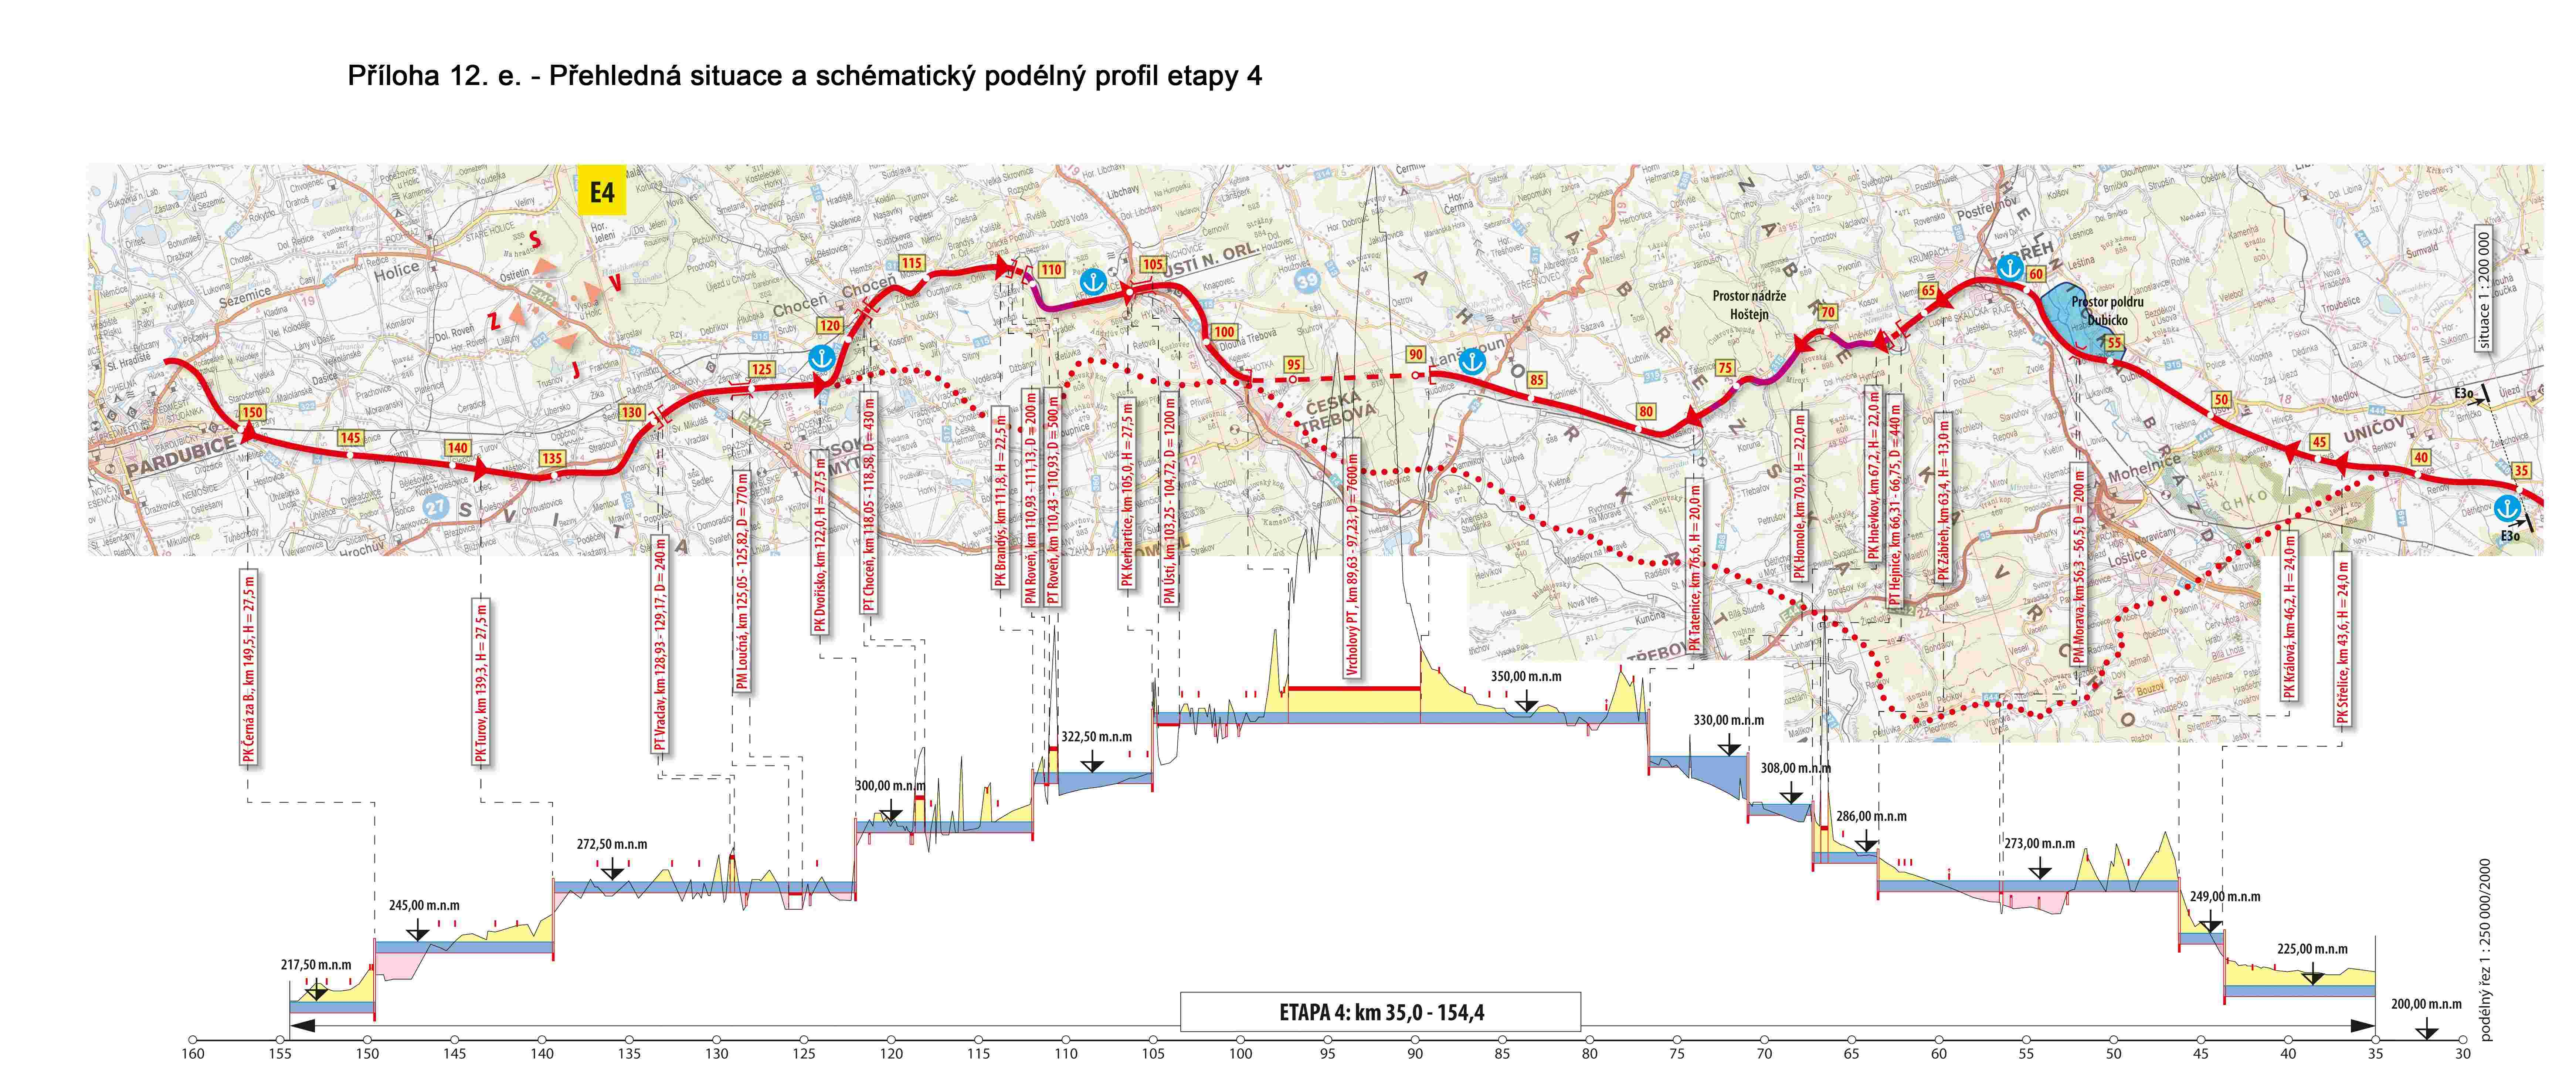
\includegraphics[width=1\textwidth, natwidth=6969, natheight=2953]
                      {etapa4.jpg}
      \caption{Ukázka jedné z části z poskytnuté literatury \label{overflow}}
    \end{figure}

    \subsection{Popis použitých technologií}

      \begin{itemize}
        \item C++ \href{http://www.cplusplus.com/}{cplusplus.com}
        \item SIMLIB
          \href{http://www.fit.vutbr.cz/~peringer/SIMLIB/}
               {www.fit.vutbr.cz/\textasciitilde peringer/SIMLIB/}
        \item g++ \href{http://www.cprogramming.com/g++.html}
                       {www.cprogramming.com/g++.html}
        \item GNU/Linux, distribuce Fedora, Ubuntu
          \href{http://fedoraproject.org/}{fedoraproject.org/},
          \href{http://ubuntu.com}{ubuntu.com}
      \end{itemize}

  \section{Koncepce modelu}

    \subsection{Forma konceptuálního modelu}


      Petriho síť na obrázku č. 2 zobrazuje mechanismus proplutí tunelu
     (stejný mechanismus lze aplikovat při proplutí mostu).
      Proměnná \texttt{M} udává počet lodí, které vplouvají do tunelu zároveň.
      Ve téměř všech tunelech je tato proměnná rovna $1$. Výjimkou je tunel
      \textit{Vrcholový}, a to kvůli své délce \,--\, 7600 metrů. U tohoto
      tunelu je proměnná \texttt{M} nastavena na hodnotu $3$, aby vzhledem k
      blízkým komorám tento tunel neměl tak značnou míru na zdržení lodí.
      Hodnota je určena na základě tabulky ve
      studii[3] (Studie projektu - stana č. 48).

      \begin{center}
        \begin{tabular}{| l | l | l | l | l | l | l | l |}
          \hline
          m & 1 & 2 & 3 & 4 & 5 & 6 & 7 \\ \hline
          $L_{mez}$ pro jednoduché pl. k. 
            & 3,47 & 6,94 & 10,42 & 13,89 & 17,36 & 20,83 & 24,30 \\ \hline
          $L_{mez}$ pro dvojité pl. k.
            & 1,63 & 3,26 &  4,88 &  6,51 &  8,14 &  9,77 & 11,40 \\ \hline
          \end{tabular}
      \end{center}

      Proměnná \texttt{T} udává čas potřebný k proplutí tunelu.
      Tento čas je určený délkou tunelu a bezpečnou
      rychlostí v těchto jednolodních tunelech, která činí
      8 km/h (Studie projektu - strana č. 47, poznámka pod čarou).
      Kvůli jednoduchosti byl zanedbán mechanismus, který je pro správné
      fungování simulace nutný \,--\, timeout. Po určité době bez proplutí lodě
      se směr tunelu automaticky změní. Doba byla navržena jako dvojnásobek
      proplouvací doby.

      \begin{figure}[ht!]
        \centering
        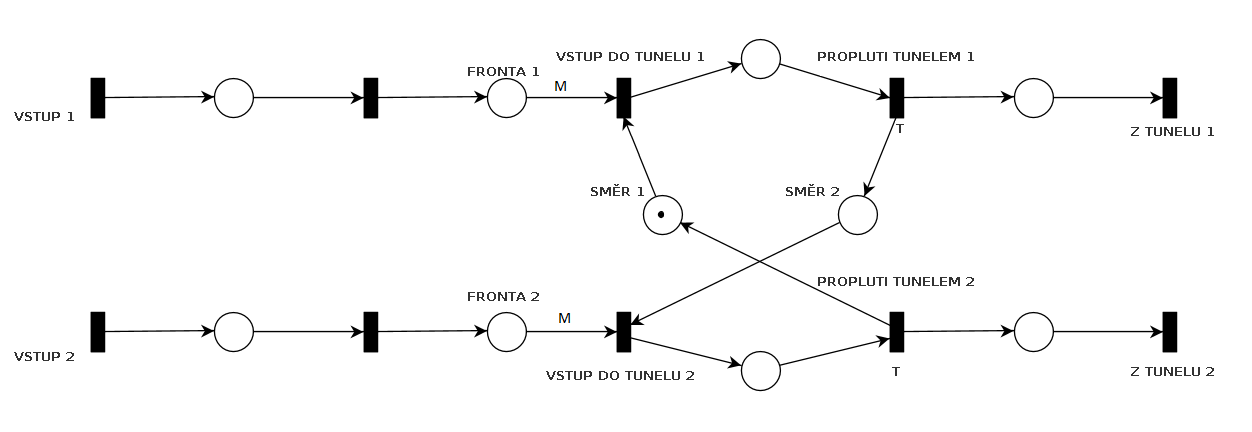
\includegraphics[width=1\textwidth, natwidth=940, natheight=325]
                        {petri_net_1.png}
        \caption{Petriho síť proplutí tunelu \label{petri_1}}
      \end{figure}

      \break

      Petriho síť na obrázku č. 3 zobrazuje mechanismus proplutí plavební
      komorou. Proměnná \texttt{X} určuje čas, za který:

      \begin{enumerate}
        \item loď vpluje do komory
        \item zavřou se vrata komory
        \item naplní se komora
        \item otevřou se vrata
        \item loď vypluje z komory
      \end{enumerate}

      Kromě naplnění komory jsou všechny konstanty získané ze
      studie[3] (Studie projektu - strana č.46-47).
      Doba napuštění (popř. vypuštění \,--\, časy jsou totožné) se odvíjí od
      výšky, kterou komora pomáhá překonávat. Doba naplnění jednoho metru v
      komoře byla zjištěna ze studie[3] (Studie projektu - strana č. 44).
      Rozlišuje se také mezi vysokými a nízkými plavebními komorami.
      Ve vysokých komorách se může voda plnit rychleji.
      Proměnná \texttt{T} udává čekací dobu, po kterou, pokud není plavební
      komora nijak využita, je komora přečerpána kvůli čekajícímu plavidlu na
      opačné hladině, než je aktuální hladina komory. Hodnotu jsme určili
      experimentováním.

      \begin{figure}[ht!]
        \centering
        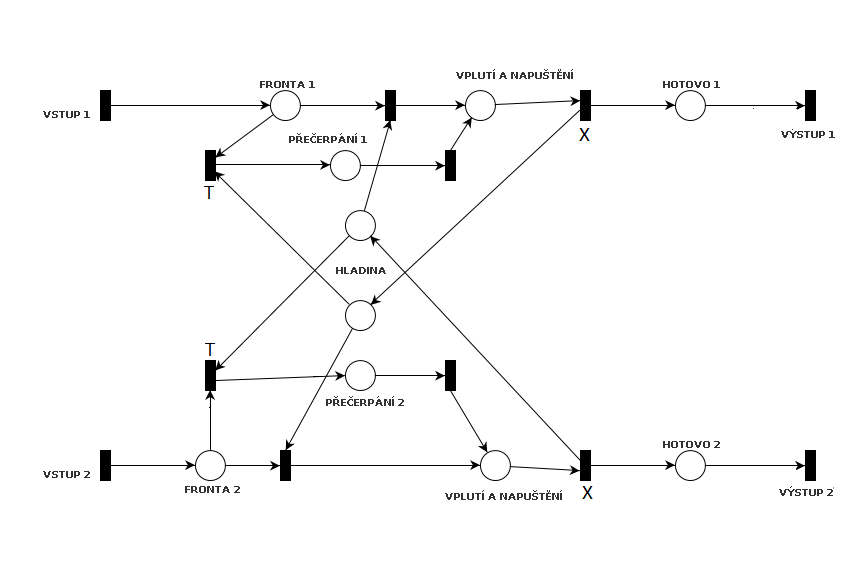
\includegraphics[width=1\textwidth, natwidth=940, natheight=325]
                        {petri_net_2.png}
        \caption{Petriho síť proplutí plavební komorou \label{petri_2}}
      \end{figure}

  \section{Závěr}

  \section{Reference}

    \begin{enumerate}[label={[\arabic*]}]
      \item Mapy s etapami výstavby koridoru 
        \href{http://d-o-l.cz/index.php/cs/kestazeni/category/14}
             {d-o-l.cz}
      % experimentalni zdroj, ale udaje souhlasi s oficialnimi
      \item Plánovaná trasa koridoru zaznačená v Google Maps
        \href{http://povode.aspone.cz/Maps/dol.html}
             {povodne.aspone.cz/Maps/dol.html}
    \end{enumerate}

  \appendix
    \newpage

  \section{Přílohy}

\end{document}
